\section{Patrones de Diseño (Facade)} 
\textbf{Tinción de fachadas derivadas de características de diseño.}\\
\begin{flushleft}
El patrón de flujo de la escorrentía de la lluvia sobre algunas características principales del diseño de la fachada de los materiales impermeables se investigó realizando simulaciones sobre ellos. Se evaluó la relación entre el patrón de flujo de escorrentía y los patrones de tinción observados. Se identificaron cuatro características principales de diseño, a saber, rebordes, desalineación de juntas, accesorios sobresalientes y unidades de persianas. Se observó que la formación de manchas era irregular y se podía determinar por el flujo de escorrentía y la acumulación de suciedad en la fachada.

\begin{itemize}
	\item Patrones de Diseño
	\\Los patrones de diseño se consideran una de las herramientas más valiosas para producir diseños de calidad y una técnica de propósito general para mejorar un diseño es identificar todas las realizaciones de patrones y aplicar reglas bien conocidas para mejorarlos..


	


	\item ¿Qué es una fachada o facade en inglés?
	\\ Es un patrón de diseño que nos permite simplificar el interface de comunicación entre dos objetos.
	\begin{center}
	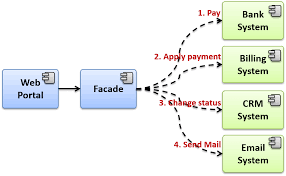
\includegraphics[width=10cm]{./images/1} 
	\end{center}

	
	\begin{center}
	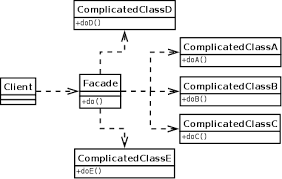
\includegraphics[width=10cm]{./images/2} 
	\end{center}


Busca simplificar el sistema, desde el punto de vista del cliente, proporcionando una interfaz unificada para un conjunto de subsistemas, definiendo una interfaz de nivel más alto. Esto hace que el sistema sea más fácil de usar.

Este patrón busca reducir al mínimo la comunicación y dependencias entre subsistemas. Para ello, utilizaremos una fachada, simplificando la complejidad al cliente. El cliente debería acceder a un subsistema a través del Facade. De esta manera, se estructura un entorno de programación más sencillo, al menos desde el punto de vista del cliente (por ello se llama "fachada").


         \item ¿Se debe utilizar cuando?
	\\ Se quiera proporcionar una interfaz sencilla para un subsistema complejo.
             Se quiera desacoplar un subsistema de sus clientes y de otros subsistemas, haciéndolo más independiente y portable.
            Se quiera dividir los sistemas en niveles: las fachadas serían el punto de entrada a cada nivel. Facade puede ser utilizado a nivel aplicación.
	\begin{center}
	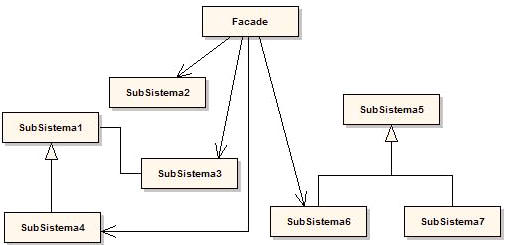
\includegraphics[width=10cm]{./images/3} 
	\end{center}

	
	

\end{itemize} 


\end{flushleft}